\documentclass[10pt]{beamer}

\usetheme{m}

\usepackage{times}
\usepackage{tikz}
\usepackage{amsmath}
\usepackage{fancyvrb}
\usepackage{xspace}

\usepackage{booktabs}
\usepackage[scale=2]{ccicons}

%\usepackage{pgfplots}
%\usepgfplotslibrary{dateplot}

\usepackage[latin1]{inputenc}
\usepackage[spanish]{babel}

\usepackage{listings}
\usepackage{pgfplots}


\title{Javascript Funcional}
\subtitle{}
\date{}
\author{Jes�s Javier Dom�nech Arellano}
\institute{27 Enero 2016}

\titlegraphic{\hfill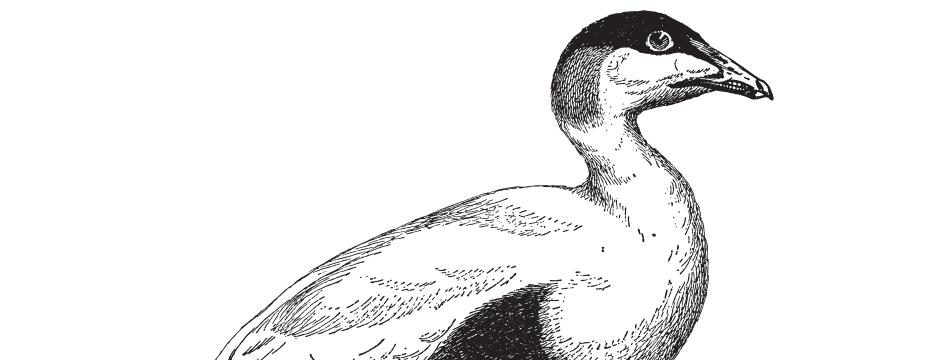
\includegraphics[scale=0.29]{images/logo.png}}

\definecolor{bgg}{HTML}{FBFBFB}
\def\gcolor{bgg}    % while presenting
%\def\gcolor{black} % while developing

\def\tikzpicdim{
  \draw[step=0.1cm, color=\gcolor] (0,0) grid (12,7);
  \draw[step=1cm, color=\gcolor] (0,0) grid (12,7);
}

\let\tikzpicdimlarge\tikzpicdim

\def\myurl{\hfil\penalty 100 \hfilneg \hbox}

\metroset{titleformat=regular}
\metroset{inner/sectiontitleformat=regular}
\metroset{outer/frametitleformat=regular}
\metroset{block=fill}


\newcommand\sectionDark[1]{{\metroset{background=dark} \section{#1} }}

%== Estilos propios de lstlisting
\lstset{%
  %backgroundcolor=\color{yellow!20},%
    basicstyle=\scriptsize\ttfamily,% breaklines=true,
    numbers=left, numberstyle=\tiny, stepnumber=1, numbersep=5pt,%
    frame=single%
    }%

% Add your keywords here, and have this in a separate file
% and include it in your preamble
%\lstset{emph={%  
%    procedure, end, to, do, pragma, omp, parallel, for, private%
%    },emphstyle={\color{black}\bfseries\underline}%
%}%



\begin{document}

\maketitle



%%======= INDICE ========================================
%\begin{frame}
%  \frametitle{�ndice}
%  \setbeamertemplate{section in toc}[sections numbered]
%  \tableofcontents[hideallsubsections]
%\end{frame}

%\section{Introduction} %=== Esrto genera una p�gina de secci�n.



\begin{frame}[fragile,fragile]
  \frametitle{Javascript}
  \begin{tikzpicture}
    \tikzpicdimlarge
    \only<1->{\node[] (def) at (0.5,6) {
        \begin{minipage}{0.9\textwidth}
          Este lenguaje posee las siguientes caracter�sticas:
          \begin{itemize}
          \item Es dinamicamente tipado.
          \item Esta orientado a objetos (prototype).
          \item Funcional.
          \item De prop�sito general.
          \end{itemize}
        \end{minipage}
      };}
    
    \only<2->{\node[] (def) at (0.5,2) {
        \begin{minipage}{0.9\textwidth}
          Adem�s, est� presente en:
          \begin{itemize}
          \item Aplicaciones m�viles.
          \item Sitios web.
          \item Servidores web.
          \item Aplicaciones de escritorio.
          \item Bases de datos.
          \end{itemize}
        \end{minipage}
      };}
  \end{tikzpicture}
\end{frame}


\begin{frame}[fragile,fragile,fragile]
  \frametitle{Expresiones}
    \begin{tikzpicture}
    \tikzpicdimlarge
    \begin{onlyenv}<1->
    \node at (0.5,6) {
      \begin{minipage}{0.9\textwidth}
        \alert{$\lambda$ expresiones:}
\begin{lstlisting}
(param1, param2, ...) => expresi�n;

(param1, param2, ...) => {
                           predicado1;
                           predicado2;
                           ...
                           return predicadofinal;
                         }
\end{lstlisting}
        \end{minipage}
      };
    \end{onlyenv}

    \begin{onlyenv}<2->
    \node at (0.5,2.4) {
      \begin{minipage}{0.9\textwidth}
        \alert{Funciones:}
\begin{lstlisting}
   function (param1, param2, ...){
      instrucci�n1;
      instrucci�n2;
      ...
      return instrucci�nfinal;
   }

   function Nombre( ... ){ ... }
\end{lstlisting}
        \end{minipage}
      };
    \end{onlyenv}    

  \end{tikzpicture}
\end{frame}

\begin{frame}[fragile]
  \frametitle{Ejemplo}

\begin{lstlisting}
    var multiplicar = (a,b) => a * b;

    var apply = (opt, a, b) => opt(a,b);
    apply(multiplicar, 4, 8); // -> 32
\end{lstlisting}
\begin{lstlisting}
    function sumar(a) {
       return function (b) {
          return a + b;
       }
    }
   
    sumar(3)(4); //-> 7
\end{lstlisting}

\end{frame}

\begin{frame}[fragile,fragile,fragile]
  \frametitle{Condicionales}
    \begin{tikzpicture}
    \tikzpicdimlarge
    \begin{onlyenv}<1->
    \node at (0.5,6) {
      \begin{minipage}{0.9\textwidth}
        \alert{Erlang:}
\begin{lstlisting}
condici�n1 -> 
              instrucciones1;
condici�n2 -> 
              instrucciones2;
...
condici�nN ->
              instruccionesN;
true       ->
              instruccionesDefault;
\end{lstlisting}
        \end{minipage}
      };
    \end{onlyenv}

    \begin{onlyenv}<2->
    \node at (0.5,3.4) {
      \begin{minipage}{0.9\textwidth}
        \alert{Operador Ternario js:}
\begin{lstlisting}
 condici�n ? instruccionesCasoCierto : instruccionesCasoFalso;
\end{lstlisting}
        \end{minipage}
      };
    \end{onlyenv}    

    \begin{onlyenv}<3->
    \node at (0.5,1.9) {
      \begin{minipage}{0.9\textwidth}
\begin{lstlisting}
 condici�n1 ? instrucciones1 : 
 condici�n2 ? instrucciones2 : 
 ...
 condici�nN ? instruccionesN : 
              instruccionesDefault;
\end{lstlisting}
        \end{minipage}
      };
    \end{onlyenv}    

  \end{tikzpicture}
\end{frame}

\begin{frame}
  \frametitle{UnderScore}
UnderScore y Lodash son dos librer�as que definen un entorno contenido
en la variable ``\_''. Nos proporciona m�todos para realizar bucles.

\begin{itemize}
\item \emph{forEach}: recibe una lista y una funci�n, se ejecuta la
  funci�n una vez por cada elemento de la lista.
\item \emph{map}: recibe una lista y una funci�n, devuelve el
  resultado de ejecutar la funci�n a cada elemento de la lista.
\item \emph{filter}: recibe una lista y una funci�n, devuelve los
  valores de la lista que dan cierto en la funci�n pasada.
\item \emph{reduce}: recibe una lista, una funci�n y un elemento
  base. La funci�n recibe un acumulador y un elemento de la
  lista. Devuelve el valor final de la acumulaci�n.
\item \emph{curry}: recibe una funci�n con N argumentos y la
  currifica.
\end{itemize}

\end{frame}



\begin{frame}
  \frametitle{�M�s? }
\begin{itemize}
\item \emph{Wrappers}
\item \emph{Funtores}
\item \emph{IO Monads}
\item \emph{Acceso al DOM}
\end{itemize}
\end{frame}

\sectionDark{Ejemplo}

%======= BIBLIOGRAF�A =======
\begin{frame}
  \frametitle{Bibliograf�a}
  
  \begin{enumerate}
  \item \url{https://dzone.com/storage/assets/379008-rc217-functionalprogramming.pdf}
  \end{enumerate}
\end{frame}

\end{document}
